\section{The automatic bridge}\label{sec:framework}
%
%The proposed bridge allows to automatically consider a UML profile as standard MOF metamodel.
%So, on one side software designers to develop models using UML profiles familiar to them, and on the other side
%developers of tools that manipulate models can assume to work on MOF metamodels only, avoiding the additional
%constraints introduced by UML profiling.

Figure~\ref{fig:overall} provides a high-level view on how the proposed bridge works. The starting point of the whole bridging mechanism is a UML profile and models conforming to it (see Figure~\ref{fig:overall}). The profile and its models can be developed using standard UML modeling tools. Then, all the other modeling artifacts involved in the bridge are automatically generated, and specifically:
\begin{enumerate}
	\item the MOF $MM$ metamodel containing all the concepts corresponding to the elements of the UML profile,
	\item a set of model-to-model transformations enabling the transformation of profiled UML models into models
conforming to the MOF metamodel, and vice versa.
\end{enumerate}


\begin{figure}[htbp]
	\centering
		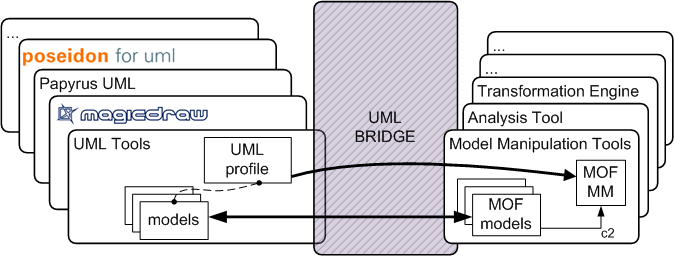
\includegraphics[width=0.85\textwidth]{figures/overview.png}
	\caption{High-level view of the proposed bridge}
	\label{fig:overall}
\end{figure}


Modeling artifacts involved in the bridging procedure lie at different levels of abstraction
(i.e., metamodeling and modeling, in the MDE modeling stack). In order to keep the bridging procedure well defined and manageable,
we decided to keep this distinction in our bridge by decomposing it into two main phases:
%
\begin{itemize}
	\item[$\bullet$] \textbf{phase 1}: it is performed at the metamodeling level, and consists in the generation of $MM$ from the UML profile.
	\item[$\bullet$] \textbf{phase 2}: it works at the modeling level, and consists in the generation of model-to-model
	transformations between UML and $MM$.
\end{itemize}

Next sections describe in details the two phases of the bridging procedure.
It is important to note that phases 1 and 2 are executed only once for each UML profile $p_x$, then generated model-to-model transformations
are re-used every time a UML model profiled with $p_x$ has to be bridged.
Furthermore, the proposed bridge is \textit{completely automatic}, i.e., when a UML profile is defined, the above mentioned bridging phases do not require any additional effort to the user. As a matter of fact, designers work on the UML side, while tool developers work on standard MOF metamodels, thus enabling a clear separation of concerns.


\subsection{Phase 1: The bridge at the metamodeling level}\label{sec:metamodelLevel}

At the metamodeling level, the bridge takes an initial UML profile and generates {\em a} corresponding MOF metamodel.
As shown in Figure~\ref{fig:metamodelingLevel}, a model-to-model transformation called
\textit{UMLprofile2MOF} is used for this purpose. This transformation generates a MOF metamodel ($MM_x$ in figure) starting from (i) the definition of the UML profile and (ii) the UML metamodel. The latter input is needed since the transformation has to access UML metaclasses referenced by the various stereotypes of the profile.

\begin{figure}[htbp]
	\centering
		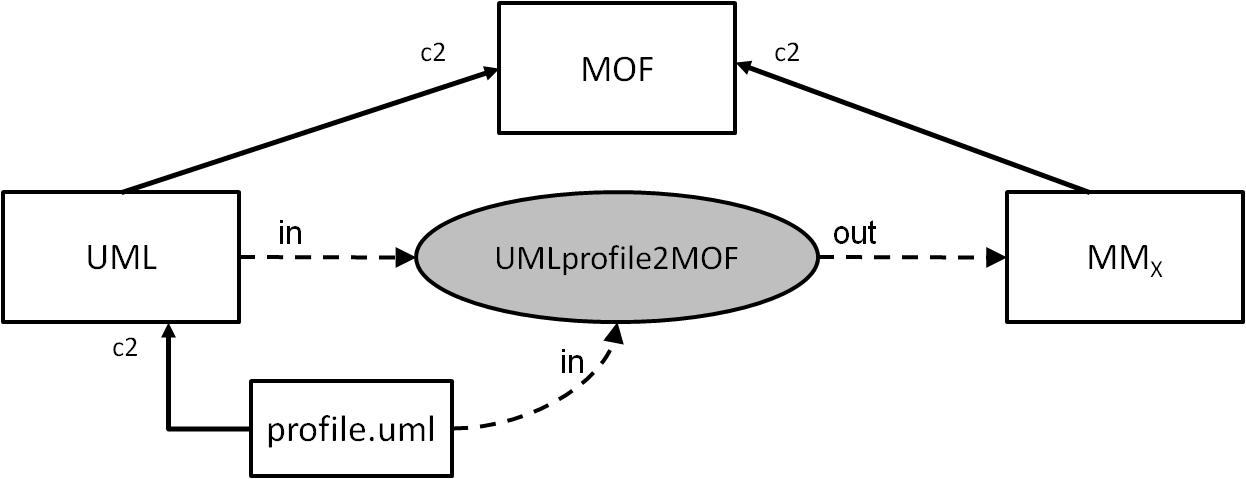
\includegraphics[width=0.60\textwidth]{figures/metamodelingLevel.png}
	\caption{The bridge at the metamodeling level}
	\label{fig:metamodelingLevel}
\end{figure}


%
The \textit{UMLprofile2MOF} transformation contains a transformation rule for each element that can appear in the definition of a UML profile. In the following we describe how the main transformation rules behave:

\begin{itemize}
	\item[$\bullet$] \textbf{Stereotype2Class}. Each UML stereotype is mapped into a MOF metaclass
	(e.g., \textit{XComponent} in Figure \ref{fig:metamodelingExample}).  		
	Tagged values of the source stereotype are separately managed by the \textit{Property2Feature} rule (described below).
	The rule also checks whether the source UML stereotype specializes some other elements, and recreates the generalization hierarchies in the target MOF metamodel, accordingly.
	A special reasoning is applied to transform the relationship between a stereotype and the UML metaclasses it extends.
	According to the UML superstructure~\cite{UML}, \textit{"the MOF construct equivalent to an extension is an aggregation from
	the extended metaclass to the extension stereotype"}. So, this rule transforms each UML extension into
	a MOF containment reference with cardinality \textit{0..1}. 	
	\item[$\bullet$] \textbf{Class2Class}, each UML class is mapped to a MOF metaclass.
	Properties of the source UML class are managed by the \textit{Property2Feature} rule and, similarly to \textit{Stereotype2Class},
	contains a specific mechanism for managing its generalization hierarchy.
	\item[$\bullet$] \textbf{Profile2Package}, each UML profile is mapped to a MOF package (e.g.,the \textit{ XProfile} in figure). Specific bindings populate the newly generated package with the correct metaclasses (generated either by the \textit{Class2Class} or the \textit{Stereotype2Class} rules) in order to recreate the same hierarchy of containments.
	\item[$\bullet$] \textbf{Package2Package}, each UML package is mapped to a MOF package. It is populated in a similar way as in the \textit{Profile2package} rule.
	\item[$\bullet$] \textbf{Property2Feature}, each UML property (like the \textit{executionTime} in figure)
	is mapped to a MOF attribute or reference depending on their type;
	more specifically, if the type of the source property is either a data type, an enumeration or a primitive type,
	then a MOF attribute is generated, otherwise the rule generates a MOF reference.
	\item[$\bullet$] \textbf{DataType2Datatype}, each UML data type is mapped to a MOF data type.
	\item[$\bullet$] \textbf{Enumeration2Enumeration}, each UML enumeration (\textit{type} in figure)
	is mapped into a MOF enumeration containing the same literals.
\end{itemize}


\begin{figure}[htbp]
	\centering
		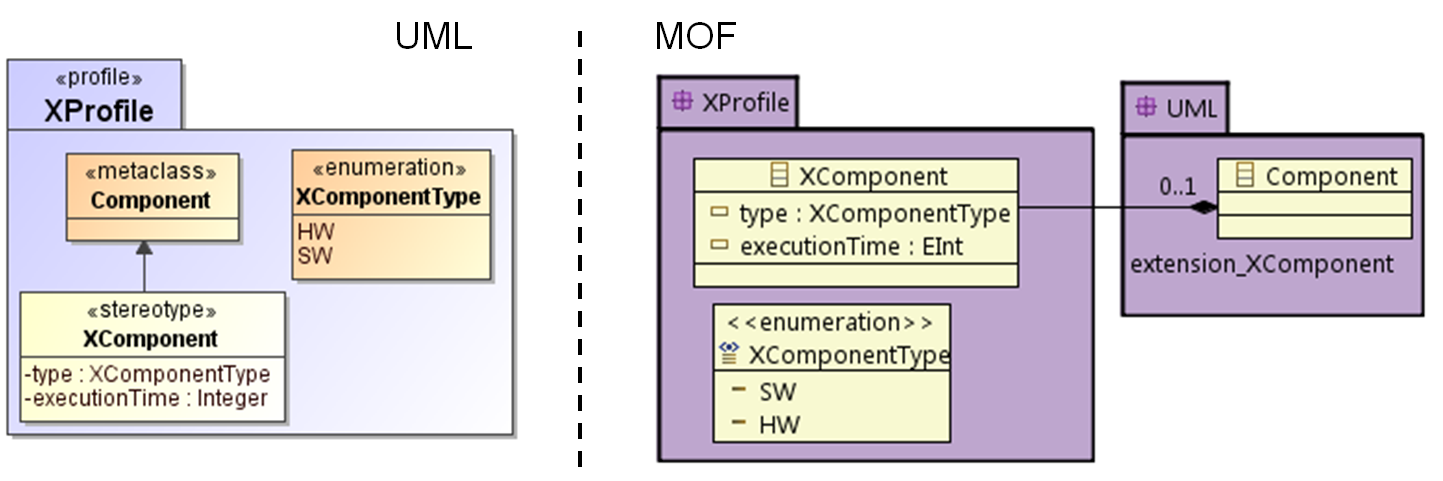
\includegraphics[width=0.70\textwidth]{figures/metamodelingExample.png}
	\caption{Example of generated MOF metamodel}
	\label{fig:metamodelingExample}
\end{figure}


\textit{UMLprofile2MOF} also contains a set of auxiliary rules and bindings (e.g., the one setting the name of each MOF meta-element with the name of the corresponding source UML element, etc.), not described in this paper for sake of simplicity. Furthermore, \textit{UMLprofile2MOF} creates an ad-hoc package in $MM_x$ where it copies all the UML metaclasses in there. In this way, the generated MOF metamodel is self-contained, and does not depend on the UML metamodel itself.
%; this opens for the possibility to "slice" the MOF metamodel, allowing to do not suffer from the complexity of the UML metamodel any more.This aspect of the bridge is presented in Section~\ref{sec:slicing}.

%Figure \ref{fig:metamodelingExample} represents a trivial UML profile translated into a MOF metamodel. The Profile has been translated into a MOF package, the Component metaclass has been copied to the target metamodel and extended through the \textit{extension\_MyStereotype} attribute. Eventually the Stereotype has been translated into a MOF metaclass and bound with the extended metaclass by means of the composition reference.
%%


\subsection{Phase 2: The bridge at the modeling level}\label{sec:modeLevel}

At the modeling level, the proposed bridge automatically generates model-to-model transformations between UML profiles and MOF metamodels.
More specifically, Figure~\ref{fig:modelingLevel} shows the two model transformations generated by our bridge:

\begin{itemize}
	\item $UML2MM_x$ returns a model conforming to $MM_x$, starting from a UML model conforming to the $profile.uml$ profile;
	\item $MM_x2UML$ performs the opposite task: it takes as input a model conforming to $MM_x$
	and produces UML models profiled according to $profile.uml$.
\end{itemize}

\begin{figure}[htbp]
	\centering
	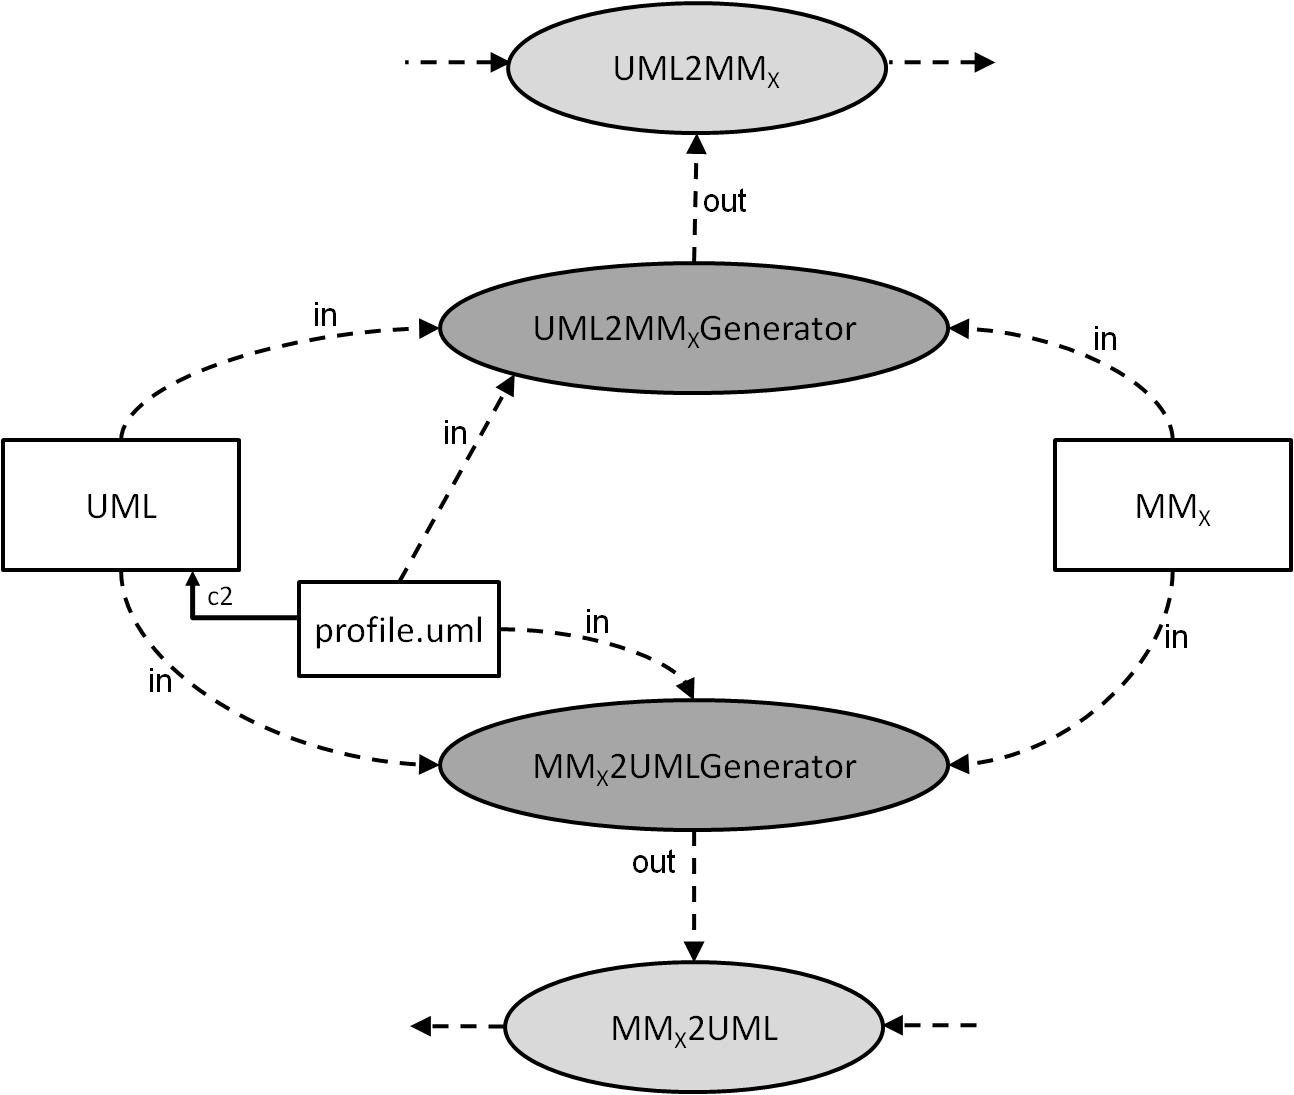
\includegraphics[width=0.60\textwidth]{figures/modelingLevel.png}
	\caption{The bridge at the modeling level}
	\label{fig:modelingLevel}
\end{figure}

$UML2MM_x$ has the following high-level logical structure: (i) a set of rules transform each standard UML element into an instance of its corresponding metaclass in $MM_x$; (ii) another set of rules transform each stereotype in the UML profile into an instance of the corresponding metaclass in $MM_x$; and (iii) for each rule, some imperative code is generated in order to automatically manage the application of stereotypes. $MM_x2UML$ works in the other way round: (i) firstly it applies the UML profile to the target UML model; (ii) then, it transforms each instance of metaclasses in $MM_x$ into an instance of the corresponding UML element; (iii) stereotypes are applied to  previously generated elements according to the definition of the UML profile. Specific rules manage the order in which profiles and stereotypes are applied, and how tagged values are accessed in the models. Figure~\ref{fig:modelingExample} shows an example of models produced by the bridge.

Such transformations are automatically generated by means of the execution of two Higher-Order Transformations
(i.e., transformations taking other transformations as input or producing
other transformations as output): $UML2MM_xGenerator$ and $MM_x2UMLGenerator$. It is important to note that higher-order transformations make the bridge generic (and so, totally automatic), so that it does not depend neither on source UML profiles nor on the generated MOF metamodels.

\begin{figure}[htbp]
	\centering
		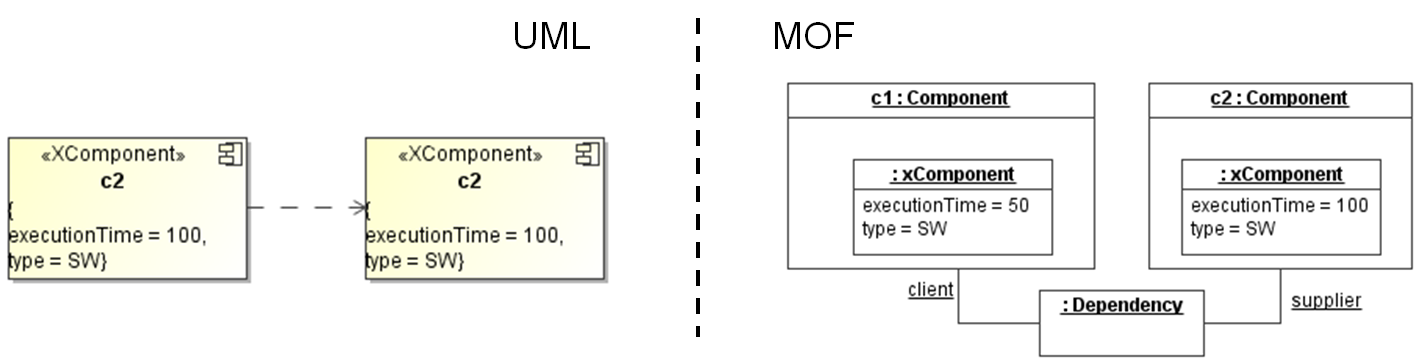
\includegraphics[width=0.70\textwidth]{figures/modelingExample.png}
	\caption{Example of bridged models}
	\label{fig:modelingExample}
\end{figure}
%

%In the figure \ref{fig:modelingExample} we show the result of the execution of the generated transformation on a model which has applied a the example profile of figure \ref{fig:metamodelingExample}. As you can see the element is a \textit{Component} and has applied \textit{MyStereotype} stereotype. In the target model we have an instance of a \textit{Component} MOF class which has an instance of a \textit{MyStereotype} class. Every tagged value has been kept and rightly instantiated.


%------------------------------------------------------------------------------------------------------------------------
\section{Slicing the obtained metamodel}\label{sec:slicing}

The default behavior of the bridge is to consider the whole UML metamodel and to keep its concepts also in the
target MOF metamodel. While ensuring loss-less transformation (and this is our primary goal while designing the bridge), our current 
approach moves the complexity of the UML metamodel (containing 246 classes and 583 properties)
into the target MOF metamodel. In order to avoid such a complexity, we couple the bridge with a \textbf{slicing mechanism} that reduces the generated metaclasses to a \textit{subset of relevant UML concepts}.

The subset of relevant UML concepts can be considered as the set of metaclasses that are expected to be instantiated
in the context of a specific project; metaclasses outside the relevant set are never instantiated in any model.
A typical example is when designers assume that they will only use, e.g., use case diagrams.
In this scenario, relevant UML concepts are only those pertaining to use case diagrams (e.g., actor, use case, association)
and there is no need to keep modeling concepts for state machines, sequence diagrams, and so on.
%This kind of assumptions is recurrent in practice, thus we designed our approach so that the target MOF metamodel contains only
%metaclasses corresponding to relevant UML concepts.
%indeed many UML modeling tools allow to restrict the kind of diagrams that can be created by designers.
%
%\begin{wrapfigure}{l}{0.45\textwidth}
	%\vspace{-20pt}
	%\begin{center}
	%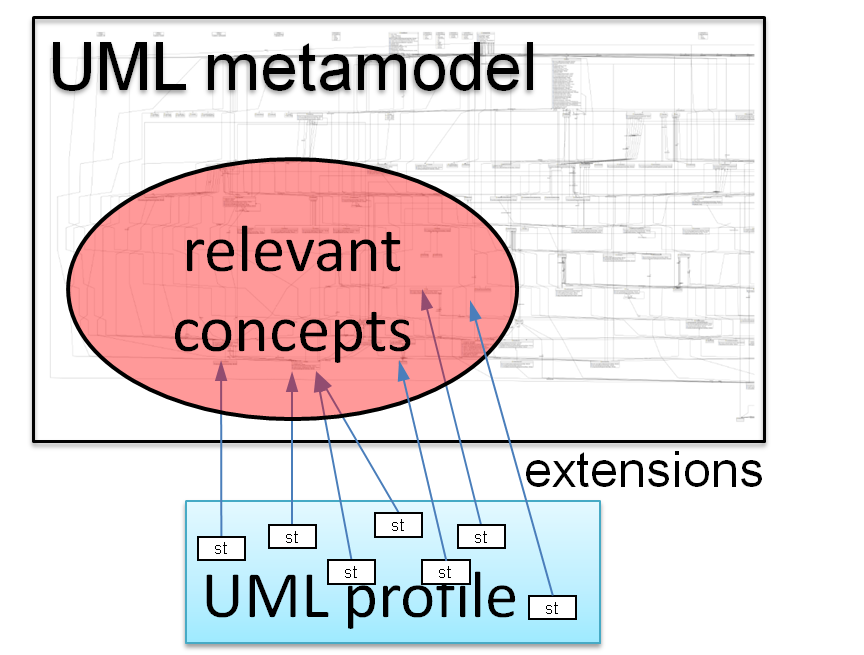
\includegraphics[width=0.44\textwidth]{figures/slicingIdea.png}
	%\end{center}
	%\caption{UML relevant concepts}
	%\label{fig:slicingIdea}
	%\vspace{-20pt}
%\end{wrapfigure}

\begin{figure}
  \centering
  \subfloat[from the UML profile]{\label{fig:slicingIdea1}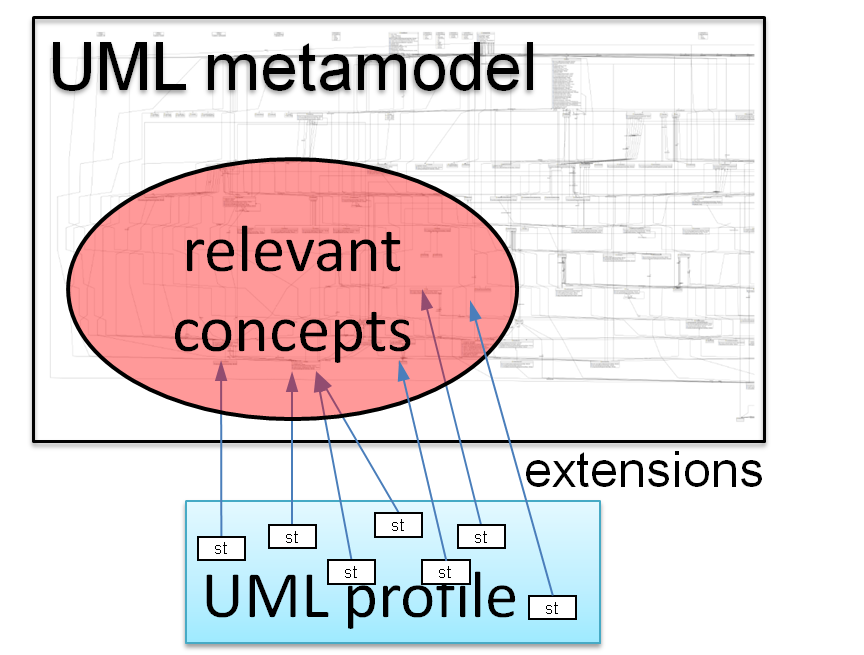
\includegraphics[scale=0.255]{figures/slicingIdea.png}}
	\hspace{2mm}
  \subfloat[from diagram names]{\label{fig:slicingIdea2}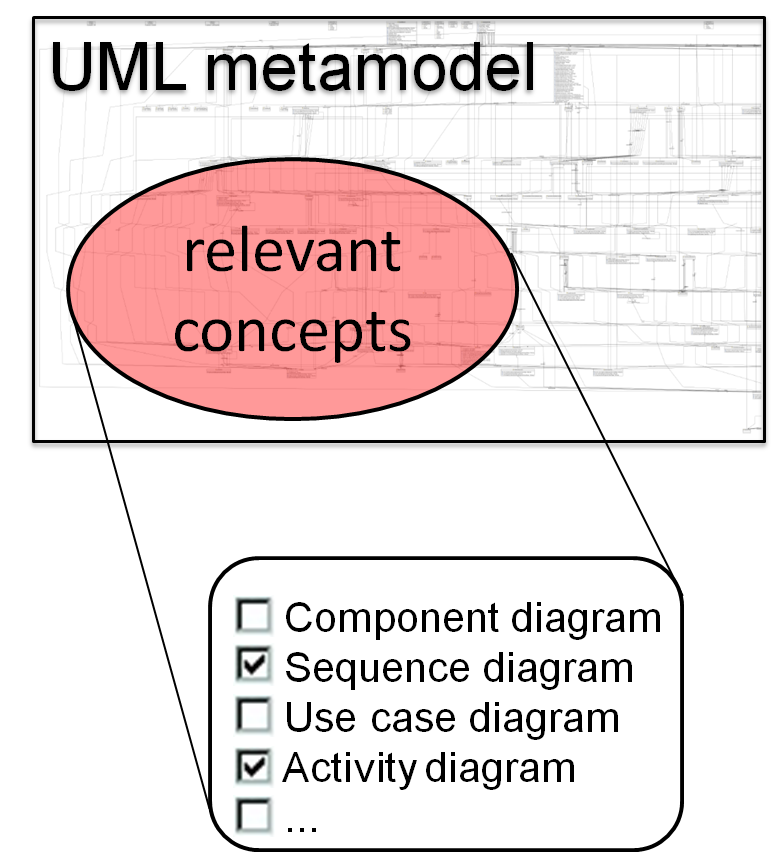
\includegraphics[scale=0.255]{figures/slicingIdea2.png}}
	\hspace{2mm}
  \subfloat[from example models]{\label{fig:slicingIdea3}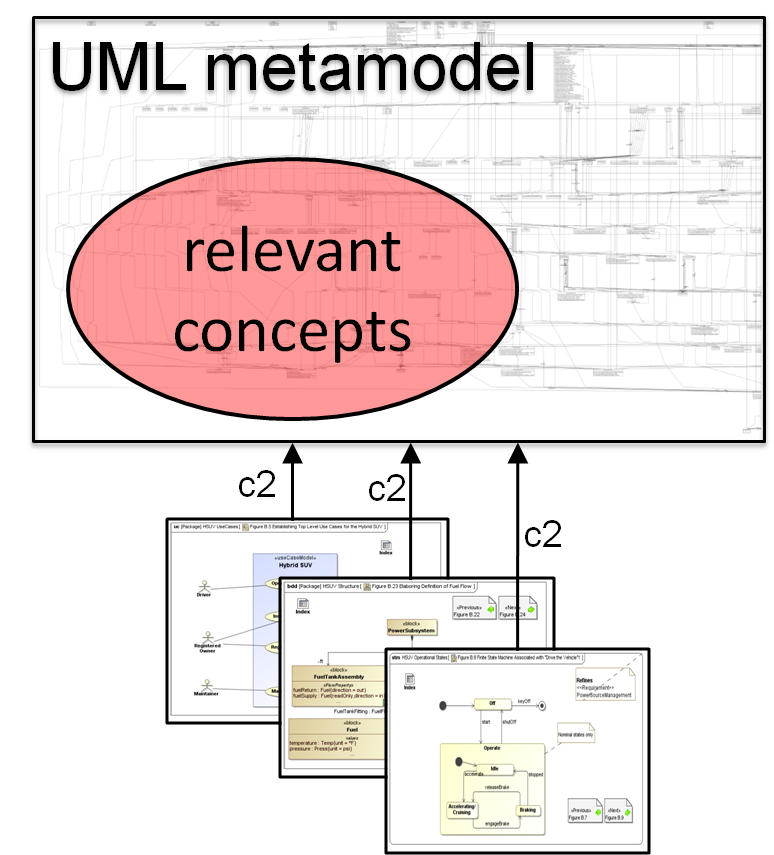
\includegraphics[scale=0.255]{figures/slicingIdea3.png}}
  \caption{Mechanisms for defining the set of UML relevant concepts}
  \label{fig:slicingIdea}
\end{figure}
%

The remainder of the section is organized as follows: firstly we describe the slicing algorithm, then we describe how sets of relevant UML concepts can be represented as annotation models, and then we will discuss how the slicing algorithm can be executed on both the target MOF metamodel and the generated model transformations.

\textbf{Slicing algorithm}. Once a set of relevant UML concepts is identifies, the slicing mechanism can be applied. Our proposal
is based and extends a generic slicing algorithm for MOF metamodels presented in~\cite{ICSEbyadl}. Intuitively,
it considers the set of relevant metaclasses and then navigates both their references and generalizations in order
to return a self-contained subset of the initial metamodel.
More formally, let $MM$ be a metamodel and let $SC$ be a subset of relevant elements in
$MM$; $slice$ is defined as follows:

\vspace{-.2cm}
$$slice(SC)=SC \cup \displaystyle\bigcup_{c \in
SC}{slice(neighbour(c))}$$
\vspace{-.2cm}

\noindent where $neighbour(c)$ is the set of all super meta-classes of
$c$, of all meta-classes referred (both with association and
aggregation) by $c$, and of all types of attributes in $c$.
It is important to note that even though $slice$ is defined
as a set of meta-classes, since each meta-class contains also references
to other meta-classes, the final result is a subset of the metamodel $MM$
with both meta-classes and their meta-relations. In this work we implemented this algorithm as a reusable library for model-to-model transformations and we adapted it in order to effectively manage the UML metamodel.\henry{non si capisce come l'approccio estende quello ICSE. Spiega meglio}

%The set of relevant metaclasses is an information related to the target MOF metamodel but it is not included in it (it depends on specific needs of designers).
\textbf{Annotation models}. Since the slicing mechanism is realized as a model transformation and considering that we were in a MDE context, the set of relevant
metaclasses is represented as an \textit{annotation model}
\footnote{An annotation model is a model containing auxiliary information about another model (the annotated model)\cite{MCDFthesis}} linked to the target MOF metamodel.
The annotation model contains a link to each relevant metaclass coming from UML, the slicing mechanism uses those links to identify the initial set of
metaclasses that will not be sliced out by the slicing procedure.
The current version of the bridge provides three mechanisms to (semi) automatically obtain the annotation model that will drive the slicing procedure:
%
\begin{enumerate}
	\item the annotation model is automatically generated from a UML profile (Figure \ref{fig:slicingIdea1}); intuitively, it creates a link in the annotation model
	for each UML metaclass extended by at least a stereotype in the profile.
	\item the GUI of the bridge allows designers to specify only the types of UML diagram they will use (e.g., activity, sequence diagrams), and the corresponding annotation model
	is automatically generated (Figure \ref{fig:slicingIdea1}); basically, designers provide the names of the UML diagrams, and this mechanism deduces the set of metaclasses belonging to those diagrams, then a link for each of those metaclasses is created in the annotation model.
	\item designers provide an example of UML model, and then the annotation model is automatically generated from it (Figure \ref{fig:slicingIdea1}).
	Basically, this mechanism checks which metaclasses are instantiated in the example model and creates a link for each found metaclass in the annotation model.
\end{enumerate}
%
These mechanisms are implemented as model transformations, each mechanism has a different level of automation and requires different input artifacts.
For example, if designers already know they will use only specific UML diagrams, then option 2 may be the most convenient;
or else, if designers already defined some initial model, they may use option 3.
Of course, if full control over the generated metamodel is needed, designers can manually define the annotation model by means of a dedicated graphical editor.
Furthermore, those mechanisms can be executed incrementally; for example a metamodel could be sliced by means of
mechanism 1, and then the resulting metamodel could be sliced multiple times with mechanism 3 with different example models;
by doing it in this way, the resulting metamodel will be more concise and accurate.
%that is they can create an annotation link for each metaclasses that can be instantiated in their UML models.

\begin{figure}
  \centering
  \subfloat[]{\label{fig:slicerMM}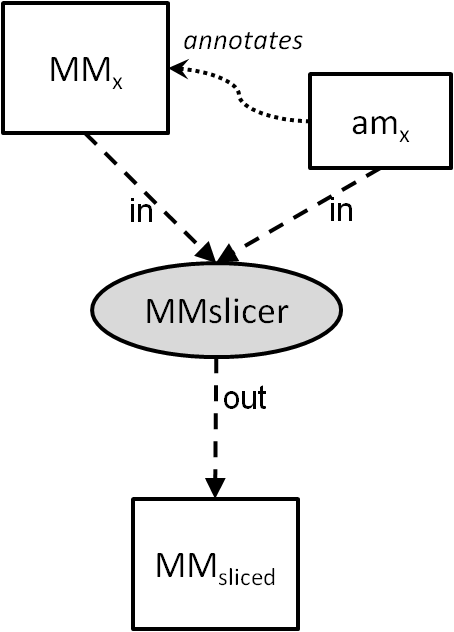
\includegraphics[scale=0.4]{figures/slicerMM}}
 \hspace{10mm}
  \subfloat[]{\label{fig:slicerT}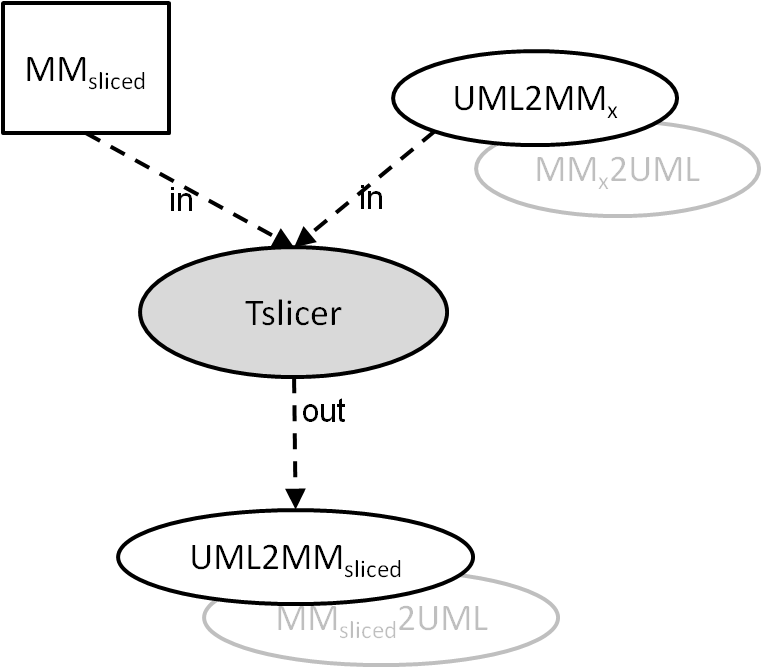
\includegraphics[scale=0.4]{figures/slicerT.png}}
  \caption{Slicing the MOF metamodel (a) and the generated transformations (b)}
  \label{fig:slicer}
\end{figure}
%
\textbf{Slicing metamodels}. As can be seen in Figure \ref{fig:slicerMM}, the slicing algorithm is used at the M2 level by a model-to-model transformation called \textit{MMslicer}.
It takes as input a MOF metamodel $MM_x$ and an annotation model $am_x$, and generates a new metamodel $MM_sliced$.
The resulting metamodel is self-contained (i.e., it does not contain any reference to external metamodels)
and contains a subset of $MM_x$ according to the metaclasses referenced in $am_x$.

At this point we must consider a possible issue that may arise: once the target MOF metamodel has been sliced, the
previously generated model transformations of the bridge may refer to missing metaclasses in the metamodel.
For example, if all the concepts related to state machines have been sliced out, the generated $UML2MM_x$ transformation still contains
transformation rules for transforming states, transitions, etc.; so, it is not aligned with the newly sliced metamodel and its execution will be erroneous.
This implies that our approach must provide a mechanism for adapting also the $UML2MM_x$ and $MM_x2UML$ transformations
to the newly sliced metamodel.
We are aware that in literature there are generic approaches managing the coupled evolution of metamodels and model transformations
\cite{TransEvolution}; however, since in our case we can assume that elements
can be only deleted from metamodels (we do not need to manage neither additions or updates), and since we need a fully automatic mechanism, we developed our minimalistic solution to automatically adapt model transformations to sliced metamodels.

\textbf{Slicing transformations}.
Our solution takes inspiration from the EMFMigrate project\footnote{EMFMigrate project website: \small{\url{http://www.emfmigrate.org}}}
and it is based on an higher-order transformation; in this work we call it $Tslicer$.
%This kind of issue is well-known in the metamodel co-evolution research field \cite{CITAZIONI}, \footnote{http://www.emfmigrate.org}
Figure \ref{fig:slicerT} gives an idea of how the \textit{Tslicer} transformation works. It takes as input (i) the sliced metamodel
($MM_sliced$ in figure) and (ii) the model transformation to be adapted ($UML2MM_x$ in figure). $Tslicer$ automatically adapts the input transformation according to the meta-elements (i.e., metaclasses, attributes, references) that were previously sliced out from $MM_sliced$.
Basically, it traverses all the instructions of the input transformation (e.g., transformation rules, assignments)
and deletes those instructions referring to meta-elements not contained into the $MM_sliced$ metamodel.
The grey elements in Figure \ref{fig:slicerT} show that $Tslicer$ can also be
applied on the transformation in the other direction (i.e., $MM_x2UML$); this ensures that using the slicing mechanism does not affect
the bridge in terms of automation and bidirectionality.
%The interested reader can refer to  details on $Tslicer$ are provided in Section \ref{sec:tool}.

In conclusion, it is important to note that the whole slicing mechanism (both on metamodels and transformations)
acts as a post-processing activity of the artifacts generated by the bridge described in Section \ref{sec:framework}; this means that, according to project-specific needs, the proposed bridge and slicing mechanism can be used independently.
%Intuitively, it copies all the elements of the input transformation (like transformation rules, imperative statements, conditions, and so on)
%and ignores those elements that reference a meta-element  that are not in $MM_sliced$ anymore.

%removes those elements of the input model transformation (e.g., transformation rules, imperative statements, conditions)
%that reference a meta-element that is not in $MM_sliced$ anymore (i.e., such an element has been sliced out by $Mslicer$).
